\documentclass[11pt]{beamer}
\usetheme{CambridgeUS}
\usepackage[utf8]{inputenc}
\usepackage[spanish]{babel}
\usepackage{amsmath}
\usepackage{amsfonts}
\usepackage{amssymb}
\author{Definición y propiedades}
\title{Integral de Riemann-Stieltjes}
%\setbeamercovered{transparent} 
%\setbeamertemplate{navigation symbols}{} 
%\logo{} 
%\institute{} 
%\date{} 
%\subject{} 
\begin{document}

\begin{frame}
\titlepage
\end{frame}

%\begin{frame}
%\tableofcontents
%\end{frame}

\begin{frame}{Particiones}

\begin{definition}
Sea $[a, b]$ intervalo. Una \textit{partición} de $[a, b]$ es un conjunto de puntos $x_0, x_1,..., x_n$ tales que
\[
	a = x_0 \leq x_1 \leq ... \leq x_n = b
\]
Sean
\[
	\Delta x_i = x_i - x_{i-1} (i = 1, ..., n)
\]
\end{definition}

\begin{center}
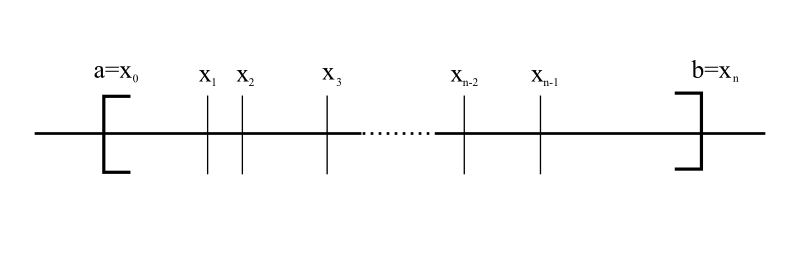
\includegraphics[scale=1]{img/particion.png}
\end{center}

\end{frame}

\begin{frame}{Integral de Riemann}



\end{frame}

\end{document}